\documentclass{article}
\usepackage{fancyhdr}
\usepackage{extramarks}
\usepackage{amsmath}
\usepackage{amsthm}
\usepackage{amsfonts}
\usepackage{tikz}
\usepackage[plain]{algorithm}
\usepackage{algpseudocode}

\begin{document}
\author{Chuan Lu}
\title{PHYS:5905 Homework 7}
\maketitle

\medskip

\begin{enumerate}
\item Problem (g)

The plot is shown in Figure \ref{problem (g)}.

\begin{figure}[h]
\centering
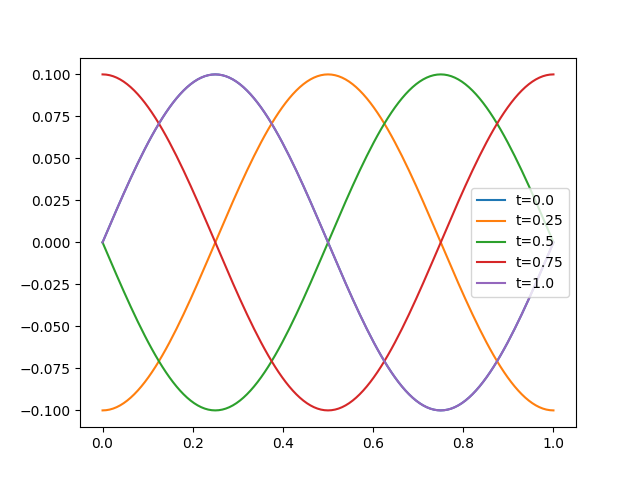
\includegraphics[scale=0.8]{problem_g.png}
\caption{$u(x) $ at $t = 0, 0.25, 0.5, 0.75, 1.0$ with $n_x = 128 $, $\Delta t = \frac{1}{128}$.}
\label{problem (g)}
\end{figure}

\item Problem (h)

The plot is shown in Figure \ref{problem (h)}.

\begin{figure}[h]
\centering
\includegraphics[scale=0.8]{problem_h.png}
\caption{$u(x)$ at $t = 0$, and at $t = 1$ with $\Delta t = \frac{1}{128}, \frac{1}{256}, \frac{1}{512}, \frac{1}{1024}$, while $n_x = 128 $.}
\label{problem (h)}
\end{figure}

I'm not sure where does the damp in the solution come from.

\item Problem (i)

The plot is shown in Figure \ref{problem (i)}.

\begin{figure}[h]
\centering
\includegraphics[scale=0.8]{problem_i.png}
\caption{$u(x)$ at $t = 0, 0.25, 0.5, 0.75, 0.8125$ with $\Delta t = \frac{1}{64}$ and $n_x = 128 $.}
\label{problem (i)}
\end{figure}

The result comes from the CFL condition:
$$
C = \frac{\Delta t}{\Delta x} = 2 > 1,
$$
so the numerical scheme is not stable.

\end{enumerate}

\end{document}